\documentclass[11pt]{article}
\usepackage{booktabs}
\usepackage{graphicx}
\usepackage{subcaption}
\usepackage{subfig}
\graphicspath{ {/home/macphej/jm.software/development/allosteric_signal/text/update_170707/figures/} }

\begin{document}
\subsection*{Testing subspace overlap implementation}
In order to test the implementation of the covariance overlap equation, which we wanted to use to measure the convergence of mutual information matrices, we calculate the time-averaged subspace overlap of positional covariance matrices of a 10 $ns$ simulation of deca-alanine peptide. We tested the accuracy of the result by calculating the same measure using the program 'gmx anaeig' in Gromacs-5.1. After fixing several indexing errors we obtained the same covariance overlap result as that calculated using the gromacs tools:
\begin{figure}[!ht]
\centering
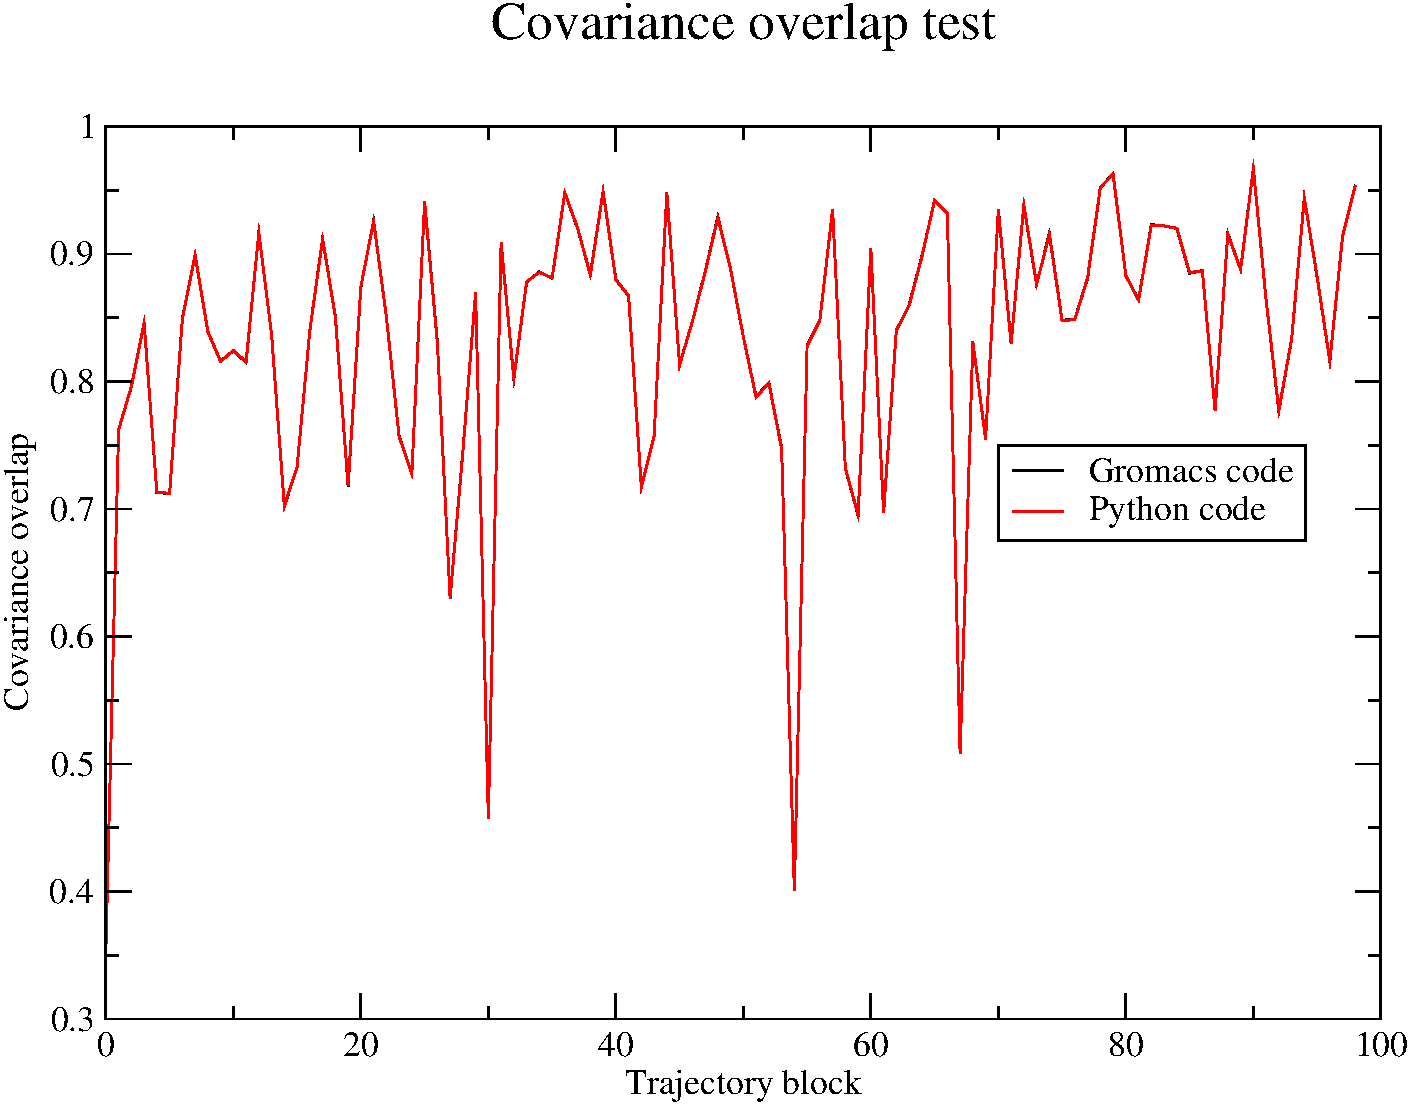
\includegraphics[scale=0.4]{decaA_code_test.pdf}
\caption{Comparison of time-averaged covariance overlap measurement with Python code and with Gromacs tools}\label{fig:1} 
\end{figure}
We obtained a perfect agreement with the covariance overlap calculated using the Gromacs tools, giving us confidence that we had implemented the algorithm accurately.

\subsection*{Measurements of positional and allosteric convergence in monomeric PKM2}
Next we investigated the degree of convergence obtained from explicit solvent simulations of monomeric PKM2 in various liganded states. For each liganded state: apo-, FBP-bound, Tepp-46-bound and L-Phe-bound- PKM2, we split the trajectory into blocks of increasing length at a fixed time window of 20 ns. From the trajectory blocks we computed the positional covariance matrix and the structural alphabet mutual information matrix. To assess the degree of convergence of positional fluctuations and allosteric transitions, respectively, we measured the covariance overlap of these two measures.
\\
\\
First, we investigated the effect of using increasing numbers of eigenmodes in the calculation of subspace overlap. For a 1 $\mu s$ explicit solvent MD simulation of monomeric PKM2 + Tepp-46, we calculated the covariance overlap for time-averaged structural alphabet mutual information.
\begin{figure}[hbt]
\centering
\begin{subfigure}[b]{.24\linewidth}
    \centering
    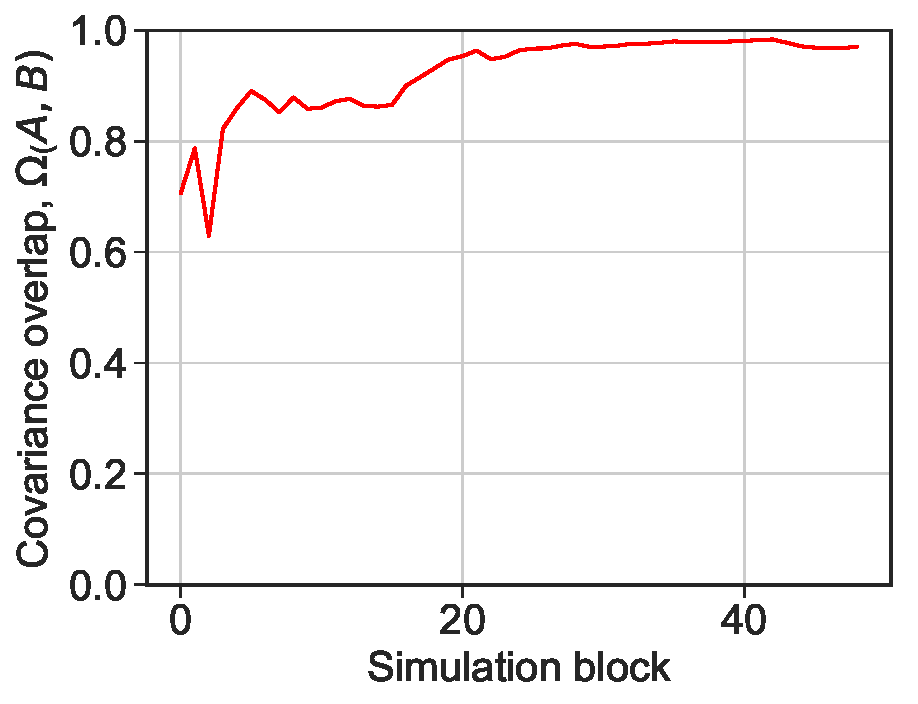
\includegraphics[width=.99\textwidth]{tepp1_MI_time_CovOver_e1.pdf}
    \caption{$E$ = 1}\label{fig:2a}
  \end{subfigure}%   
  \begin{subfigure}[b]{.24\linewidth}
    \centering
    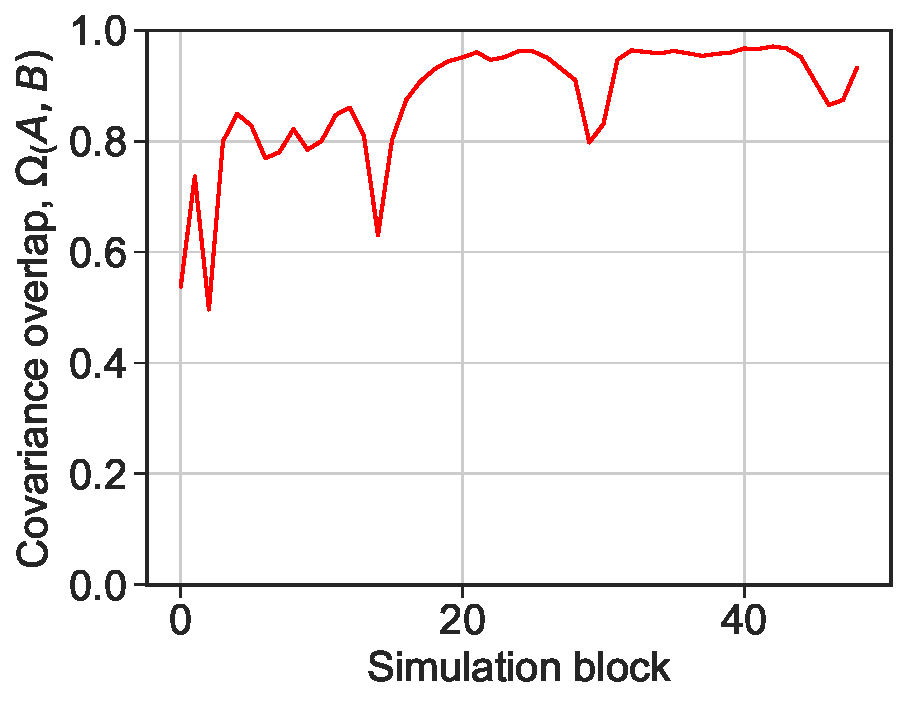
\includegraphics[width=.99\textwidth]{tepp1_MI_time_CovOver_e2.pdf}
    \caption{$E$ = 2}\label{fig:2b}
  \end{subfigure}%  
  \begin{subfigure}[b]{.24\linewidth}
    \centering
    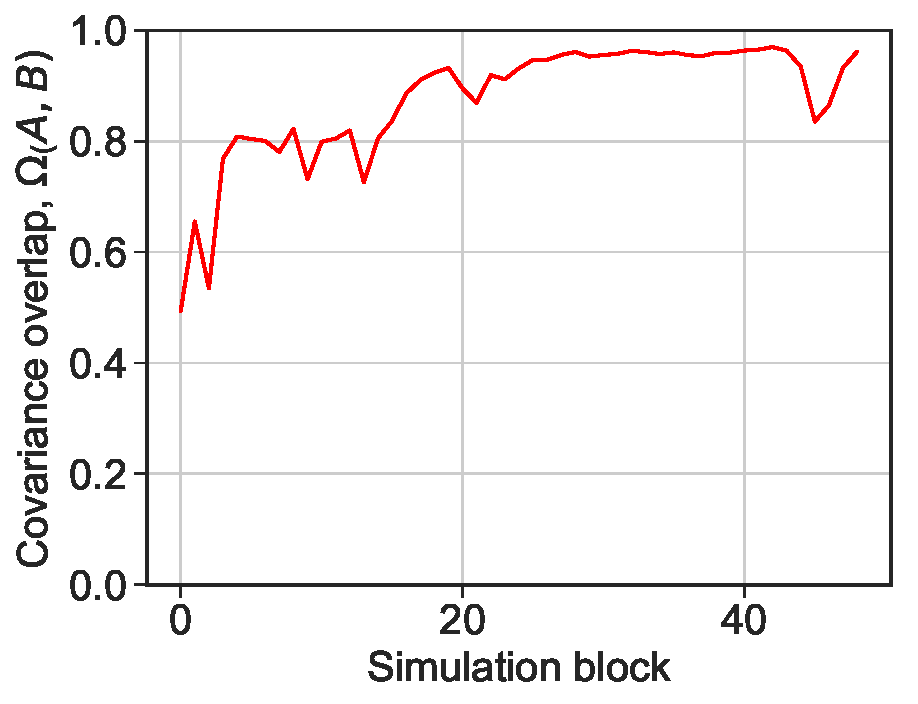
\includegraphics[width=.99\textwidth]{tepp1_MI_time_CovOver_e3.pdf}
    \caption{$E$ = 3}\label{fig:2c}
  \end{subfigure}%  
  \begin{subfigure}[b]{.24\linewidth}
    \centering
    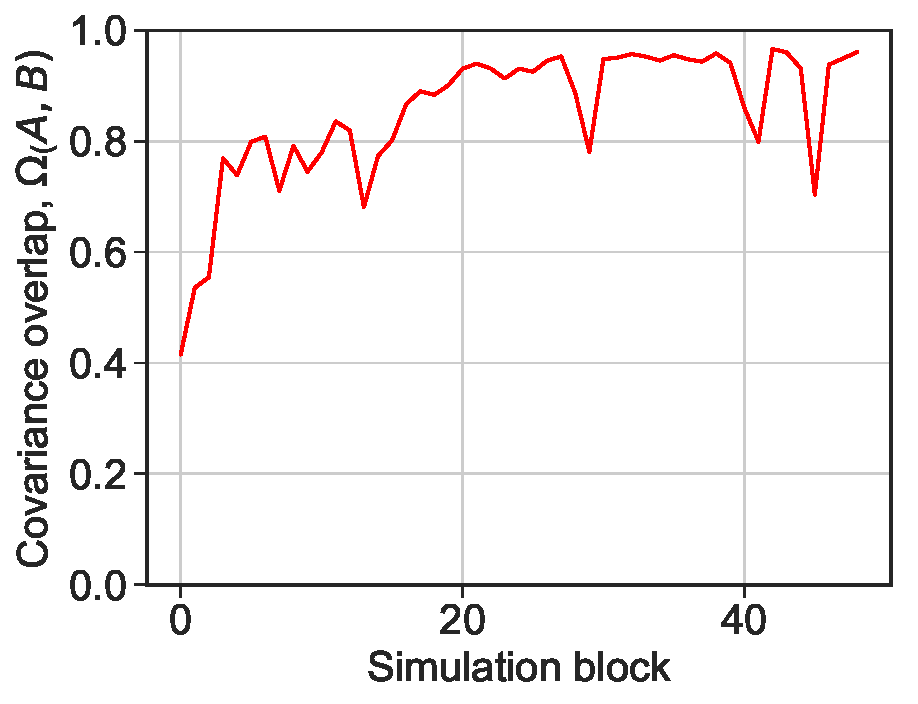
\includegraphics[width=.99\textwidth]{tepp1_MI_time_CovOver_e4.pdf}
    \caption{$E$ = 4}\label{fig:2d}
  \end{subfigure}\\%   
  \begin{subfigure}[b]{.24\linewidth}
    \centering
    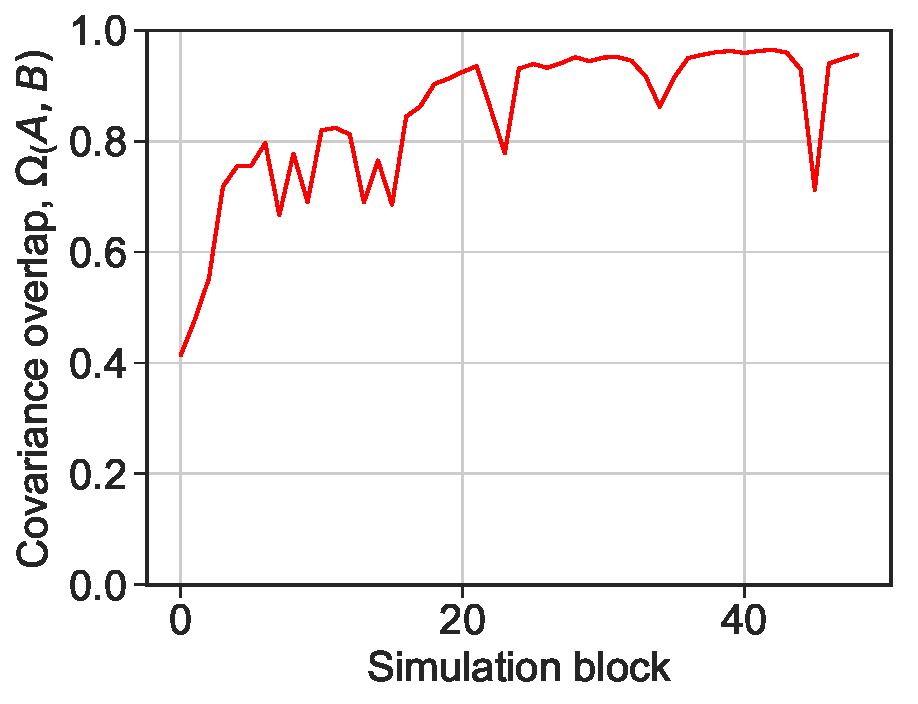
\includegraphics[width=.99\textwidth]{tepp1_MI_time_CovOver_e5.pdf}
    \caption{$E$ = 5}\label{fig:2e}
  \end{subfigure}%
  \begin{subfigure}[b]{.24\linewidth}
    \centering
    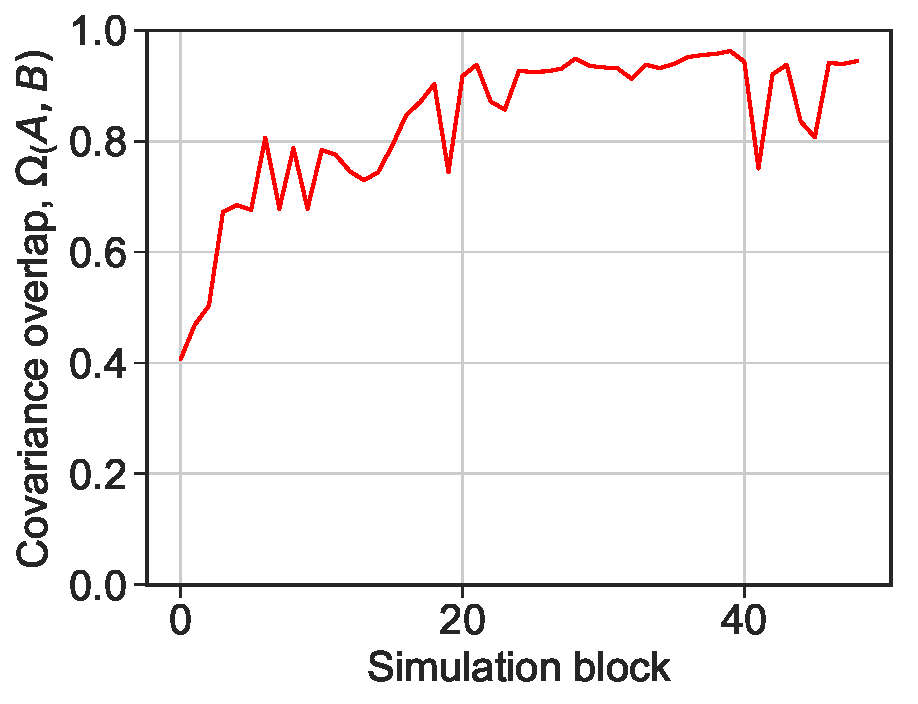
\includegraphics[width=.99\textwidth]{tepp1_MI_time_CovOver_e6.pdf}
    \caption{$E$ = 6}\label{fig:2f}
  \end{subfigure}%
  \begin{subfigure}[b]{.24\linewidth}
    \centering
    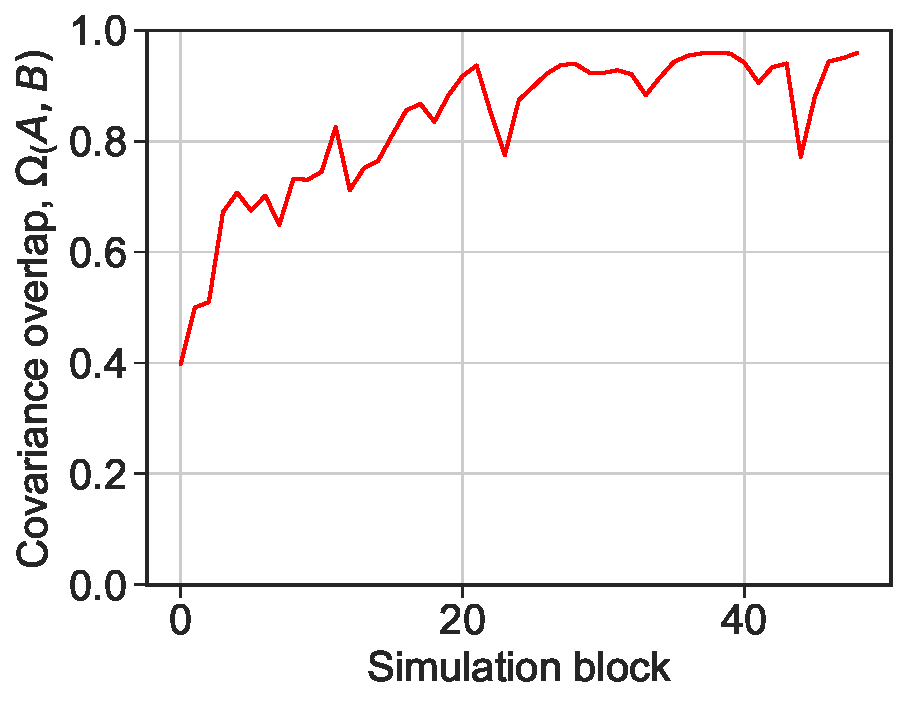
\includegraphics[width=.99\textwidth]{tepp1_MI_time_CovOver_e7.pdf}
    \caption{$E$ = 7}\label{fig:2g}
  \end{subfigure}%
  \begin{subfigure}[b]{.24\linewidth}
    \centering
    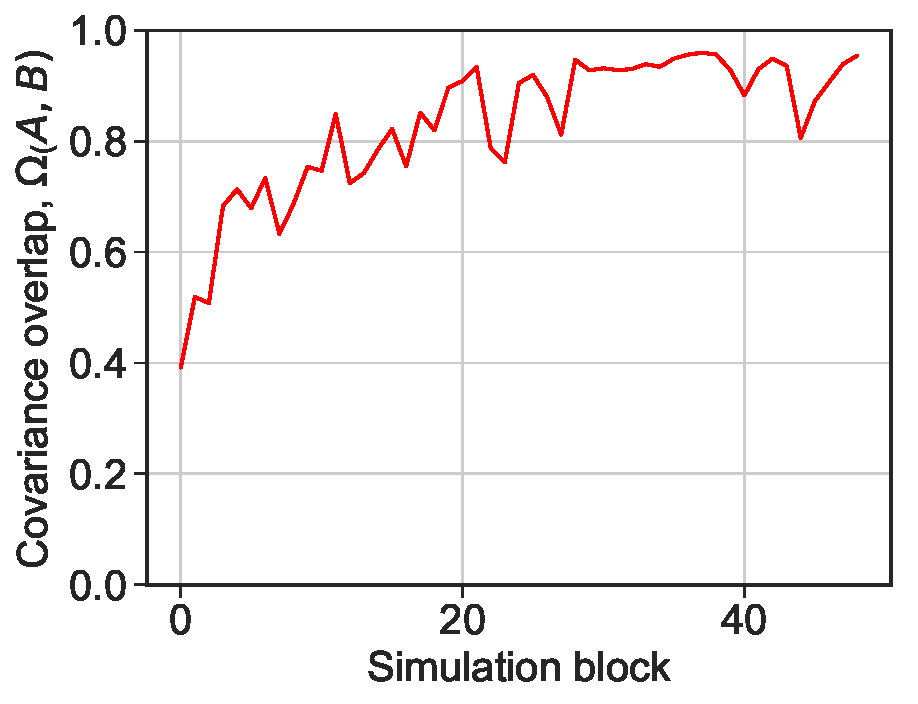
\includegraphics[width=.99\textwidth]{tepp1_MI_time_CovOver_e8.pdf}
    \caption{$E$ = 8}\label{fig:2h}
  \end{subfigure}\\%     
  \begin{subfigure}[b]{.24\linewidth}
    \centering
    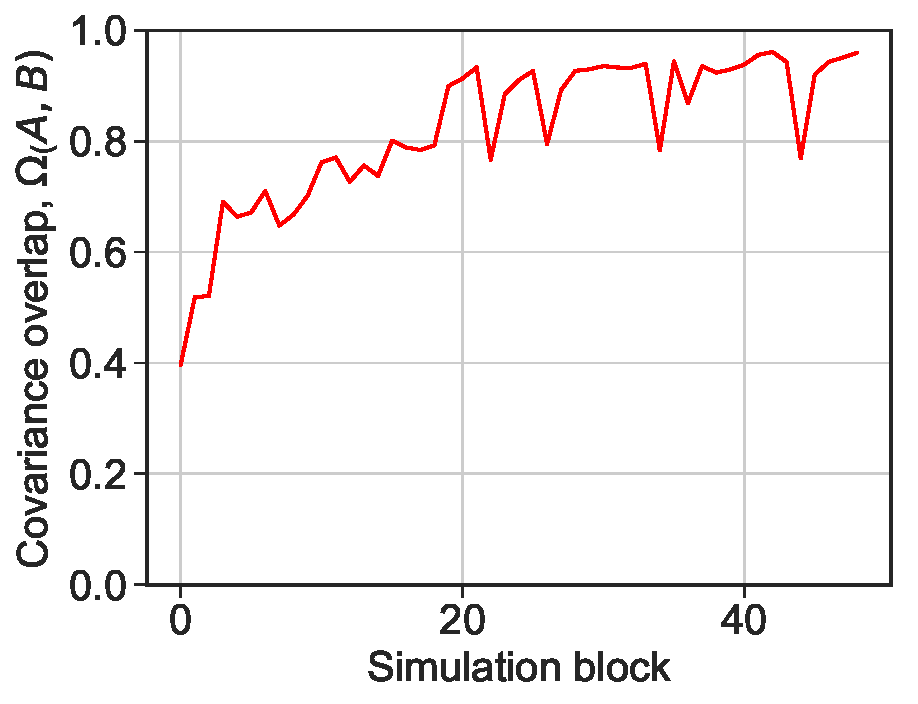
\includegraphics[width=.99\textwidth]{tepp1_MI_time_CovOver_e9.pdf}
    \caption{$E$ = 9}\label{fig:2i}
  \end{subfigure}%
  \begin{subfigure}[b]{.24\linewidth}
    \centering
    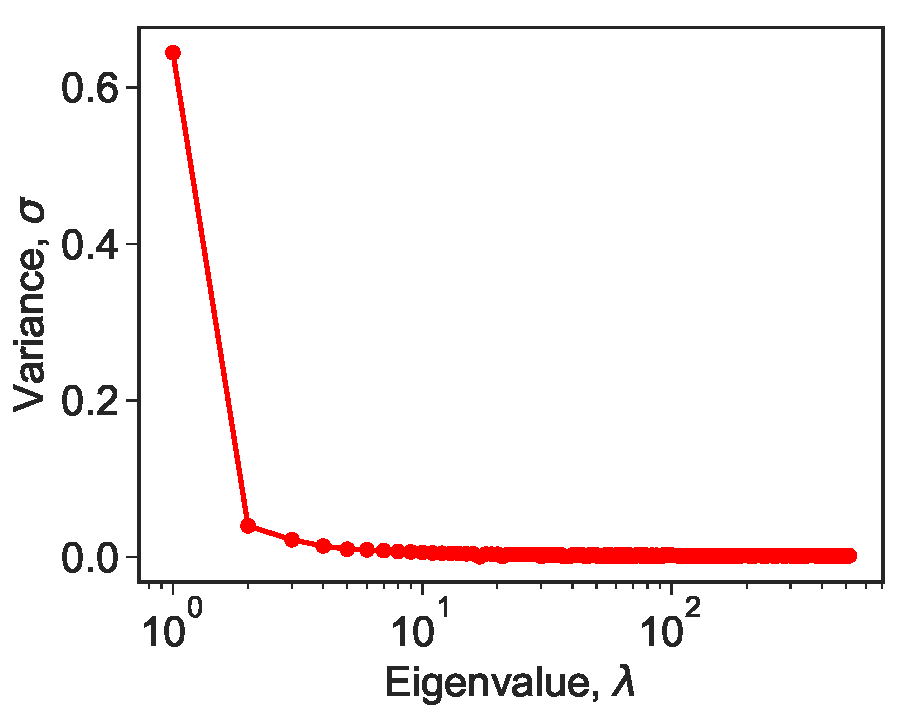
\includegraphics[width=.99\textwidth]{tepp1_MI_screeplot.pdf}
    \caption{Scree plot}\label{fig:2j}
  \end{subfigure}%
\caption{The numerical behaviour of covariance overlap with different eigenmodes for monomeric PKM2 + Tepp-46. The MD trajectory was split into 50 sliding windows with a length of 20 $ns$. The subspace overlap was calculated for each blocks $i_{n}$ and $i_{n-1}$}\label{fig:2}
\end{figure}
Qualitatively, we observed a convergent effect on the shape of the covariance overlap curve with increasing number of eigenmode, though a Scree plot suggested that only the first eigenmode contributed any appreciable variance following the spectral decomposition. To see whether inclusion of different numbers of eigenmodes in the time-averaged covariance overlap measurement we fitted the curves to a two-exponental regression. Autocorrelation functins of principal components can be fitted with a double exponential function using a fast and slow correlation time. Within a conformational state there is a short correlation time as the local well(s) are explored. The transition between different conformations occurs on slower timescales, which is captured by the second term. We found no meaningful correlation between either rate terms and the eigenmode number. It should be noted that the time-averaged covariance overlap for $\lambda=2$ was not possible to fit to the exponental regression.
\begin{table}[!ht]
\centering
\caption{Fitting of two-exponential curve to covariance overlap for different eigenmodes, mutual information matrix for monomeric PKM2 + Tepp-46.}
\label{Table 1}
\begin{tabular}{@{}lll@{}}
\toprule
$\lambda$ & $t_1$ ($ns$) & $t_2$ ($ns$) \\ \midrule
1         & 28.88         & 209.2        \\
2         & N.A           & N.A          \\
3         & 17.13         & 184.7        \\
4         & 18.56         & 164.34       \\
5         & 20.40         & 212.2        \\
6         & 22.18         & 161.38       \\
7         & 16.81         & 175.32       \\
8         & 16.87         & 200.60       \\
9         & 13.74         & 214.80       \\ \bottomrule
\end{tabular}
\end{table} 
To determine whether the convergence of positional fluctuations captured by the $C_\alpha$ covariance matrix coinsided with the convergence of the structural alphabet mutual information matrix, we compared the time-averaged covariance overlap for these two measures for a $1 \mu s$ simulation of monomeric PKM2 + Tepp-46.
\begin{figure}[!ht]
\centering
\begin{subfigure}[b]{.4\linewidth}
    \centering
    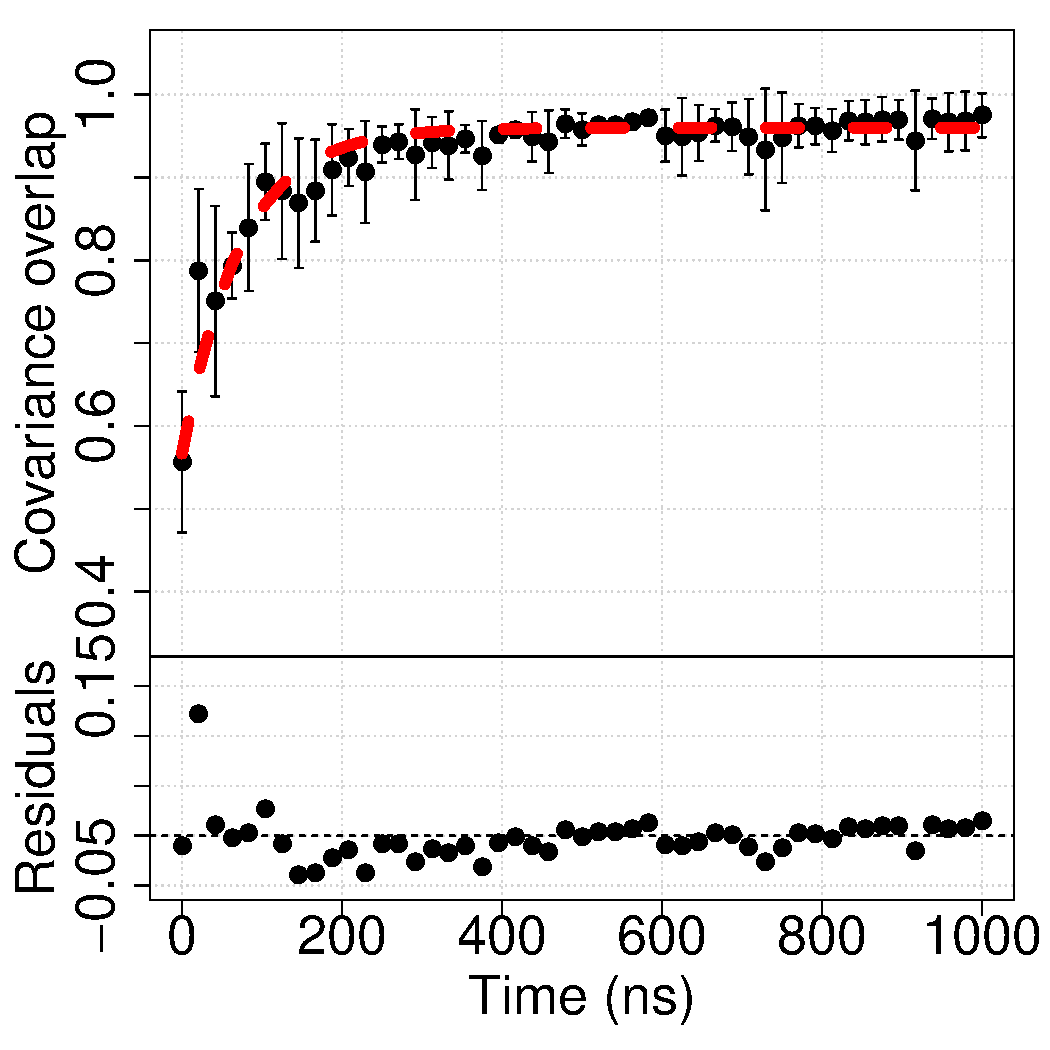
\includegraphics[width=.99\textwidth]{pos_overlap_tepp.pdf}
    \caption{$C_\alpha$ positional covariance}\label{fig:3a}
  \end{subfigure}%   
  \begin{subfigure}[b]{.4\linewidth}
    \centering
    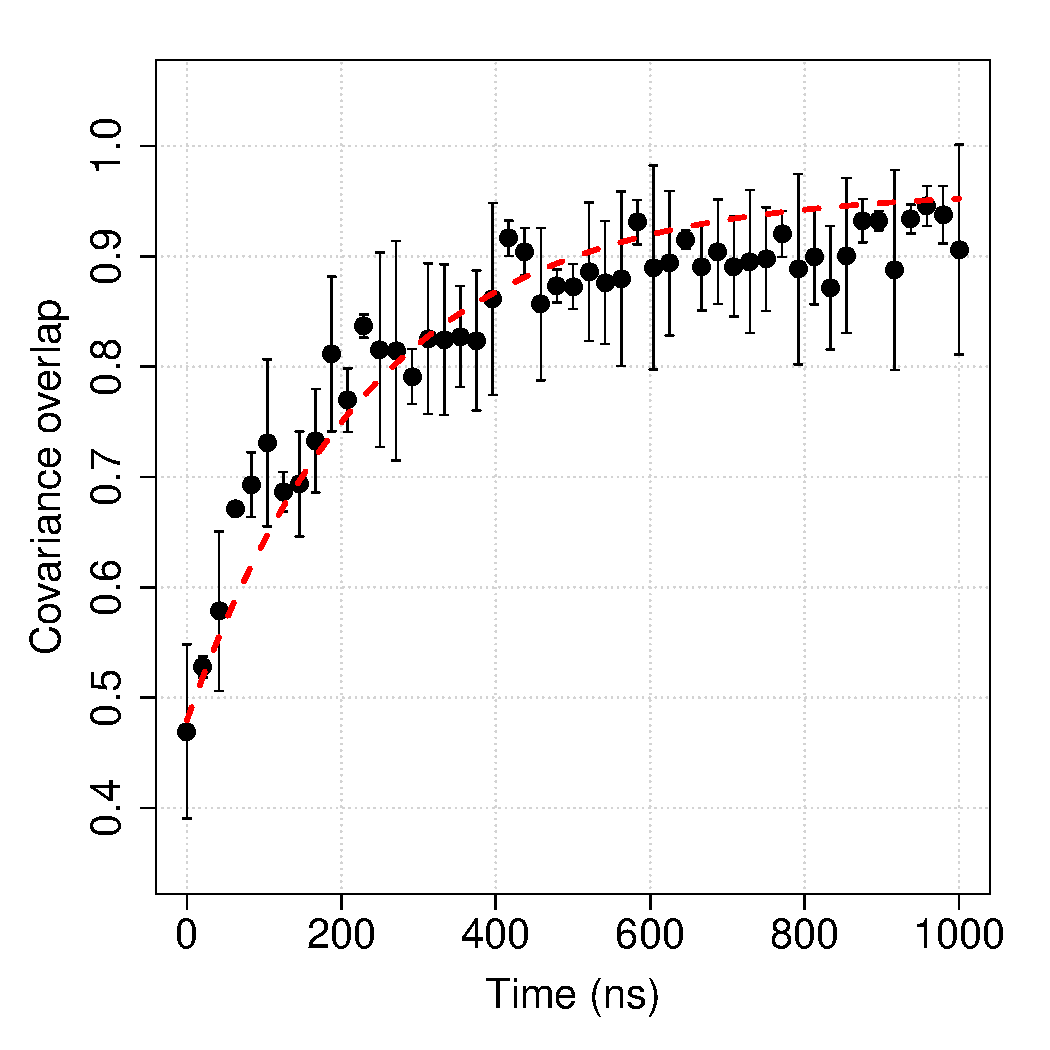
\includegraphics[width=.99\textwidth]{MI_overlap_tepp.pdf}
    \caption{Mutual information}\label{fig:3b}
  \end{subfigure}%  
  \begin{subfigure}[b]{.4\linewidth}
    \centering
    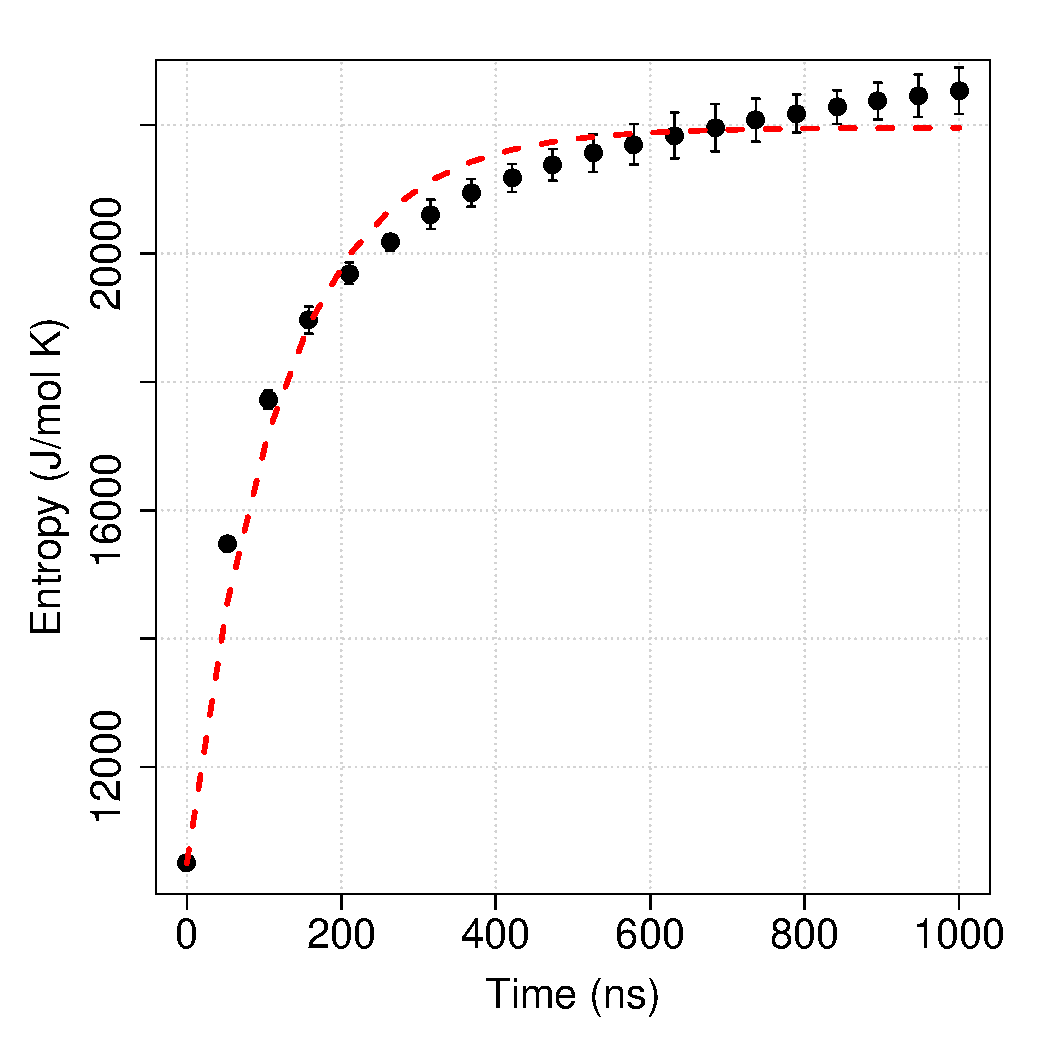
\includegraphics[width=.99\textwidth]{tepp_entropy.pdf}
    \caption{Entropy}\label{fig:3b}
  \end{subfigure}%  
\caption{Energetic and structural features of monomeric PKM2 + Tepp-46 equilibration. Comparison of the time-averaged covariance overlap for the (a) $C_\alpha$ covariance matrix and the (b) structural alphabet mutual information matrix. The first ten eigenmodes were used in calculating covariance overlap for both (a) and (b). (c) Time-averaged configurational entropy measured over the course of the MD simulation.}\label{fig:2}
\end{figure}
A two-exponential fit of the curves in figure 3a and 3b revealed quantitative differences between the two measures of structural relaxation. The covariance overlap of the mutual information matrix yielded a fast relaxation time ($t_1$) of $28.8$ $ns$ and a slow relaxation time ($t_2$) of $174.2$ $ns$. Both the ($t_1$) and ($t_2$) values for the $C_\alpha$ positional covariance matrix were significantly shorter $0.1$ $ns$ and $90.1$ $ns$, respectively.
\\
\\
Longer relaxation rates estimated from the structural alphabet mutual information matrix compared to the $C_\alpha$ positional covariance matrix suggests that backbone conformational changes, captured by the structural alphabet, take much longer to equilibrate than the fast vibrations of the protein backbone. The long relaxation rate ($t_2$) may also provide an indication of the timescale on which allosteric transitions occur in PKM2 upon Tepp-46 binding. Still longer relaxation kinetics were observed when the energetic evolution of the MD trajectory was considered with configurational entropy: $t_1$ $=$ $41.3$ $ns$ and $t_2$ $=$ $272.4$ $ns$. These three measurements reveal three distinct timescales of protein dynamics; fast-timescale $C_\alpha$ positional vibrations, backbone conformational, and configurational energetic changes.
\begin{figure}[!ht]
\centering
\begin{subfigure}[b]{.4\linewidth}
    \centering
    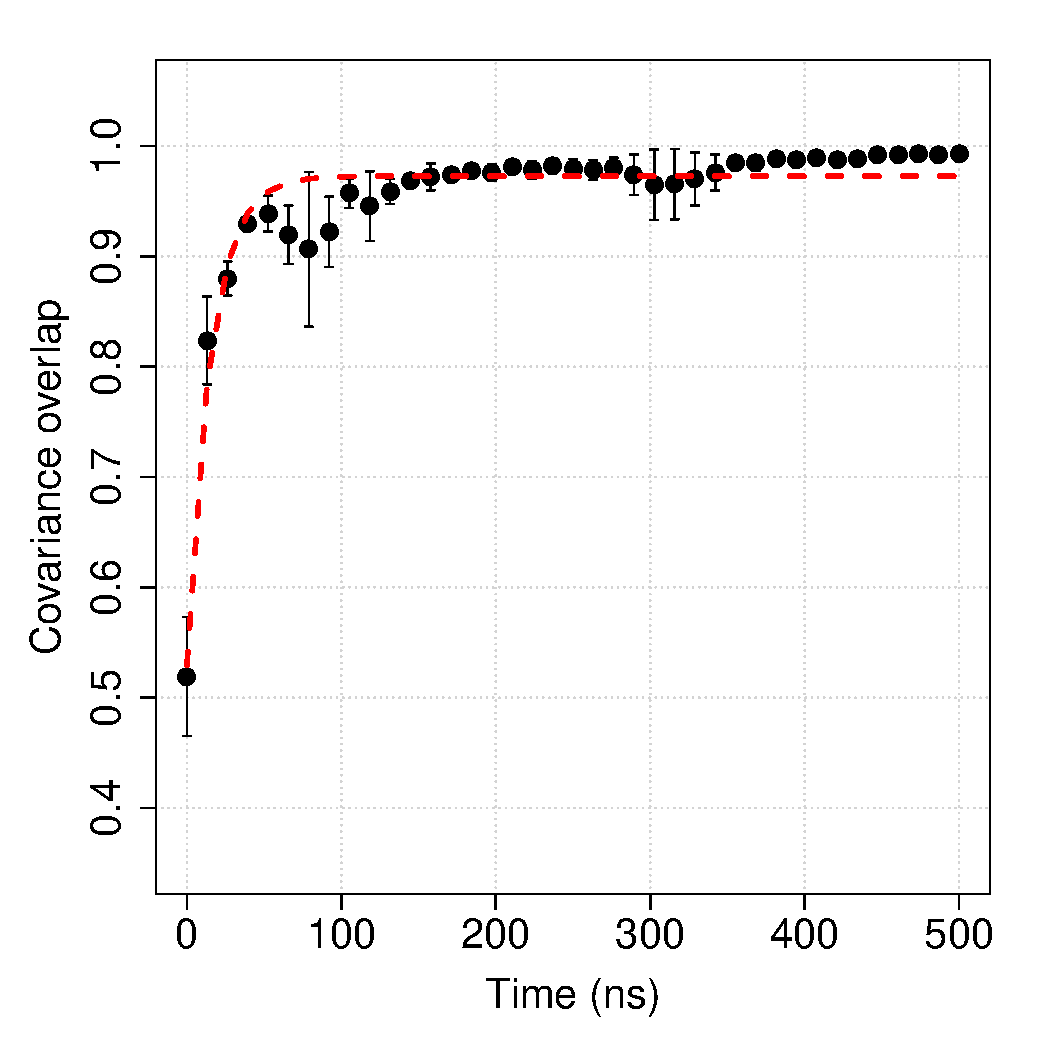
\includegraphics[width=.99\textwidth]{pos_overlap_fbp.pdf}
    \caption{$C_\alpha$ positional covariance}\label{fig:4a}
  \end{subfigure}%   
  \begin{subfigure}[b]{.4\linewidth}
    \centering
    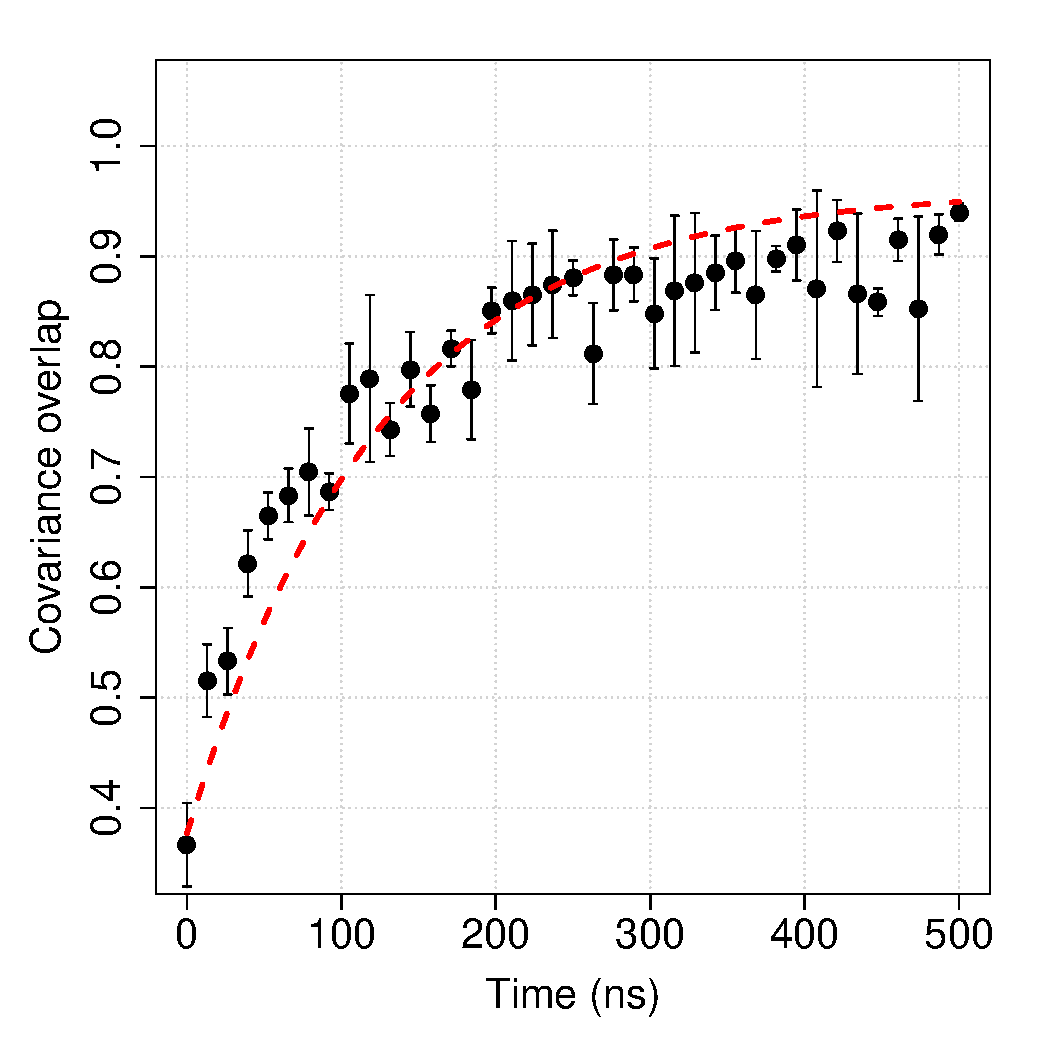
\includegraphics[width=.99\textwidth]{MI_overlap_fbp.pdf}
    \caption{Mutual information}\label{fig:3b}
  \end{subfigure}%  
  \begin{subfigure}[b]{.4\linewidth}
    \centering
    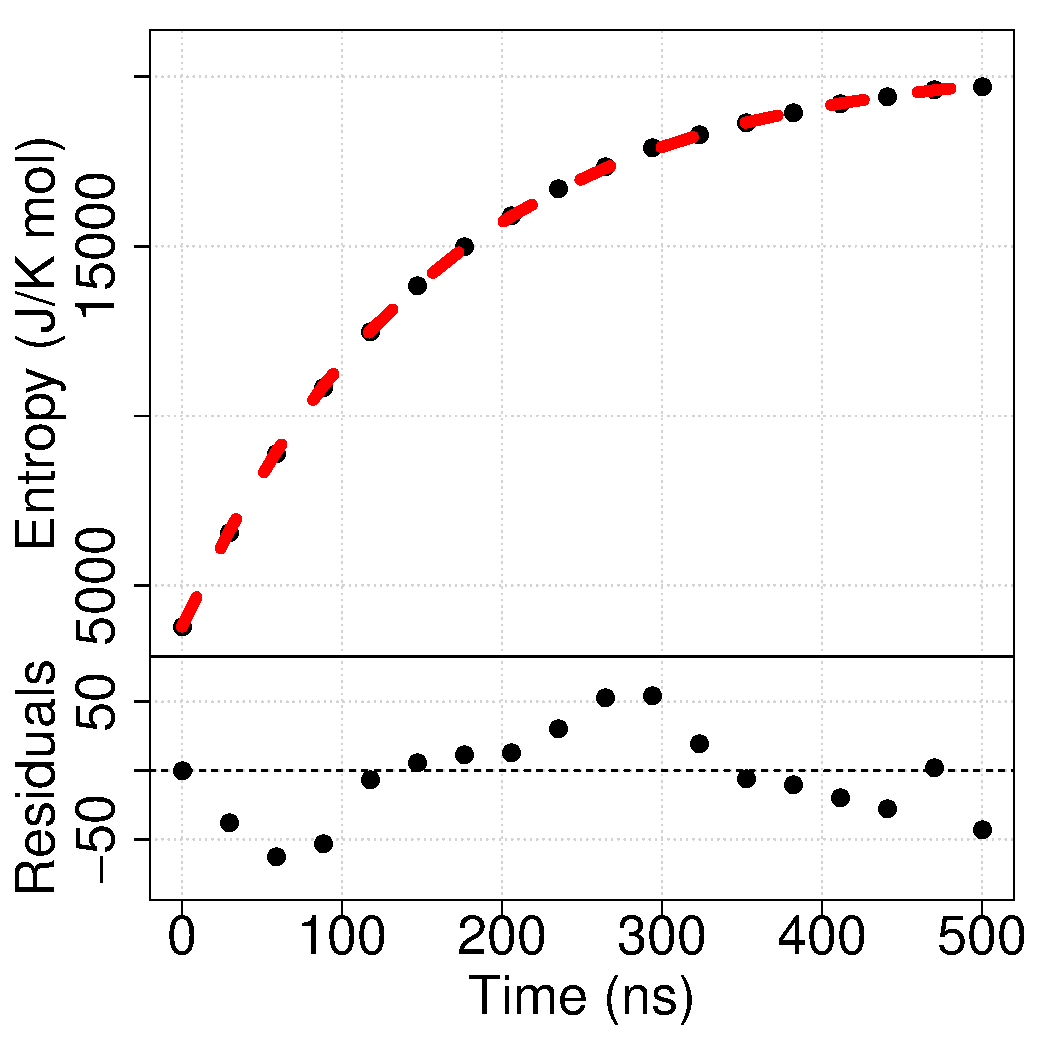
\includegraphics[width=.99\textwidth]{entropy_fbp.pdf}
    \caption{Entropy}\label{fig:3b}
  \end{subfigure}%  
\caption{Energetic and structural features of monomeric PKM2 + fructose-1,6-bisphosphate equilibration. Comparison of the time-averaged covariance overlap for the (a) $C_\alpha$ covariance matrix and the (b) structural alphabet mutual information matrix. The first ten eigenmodes were used in calculating covariance overlap for both (a) and (b). (c) Time-averaged configurational entropy measured over the course of the MD simulation.}\label{fig:2}
\end{figure}
\begin{figure}[!ht]
\centering
\begin{subfigure}[b]{.4\linewidth}
    \centering
    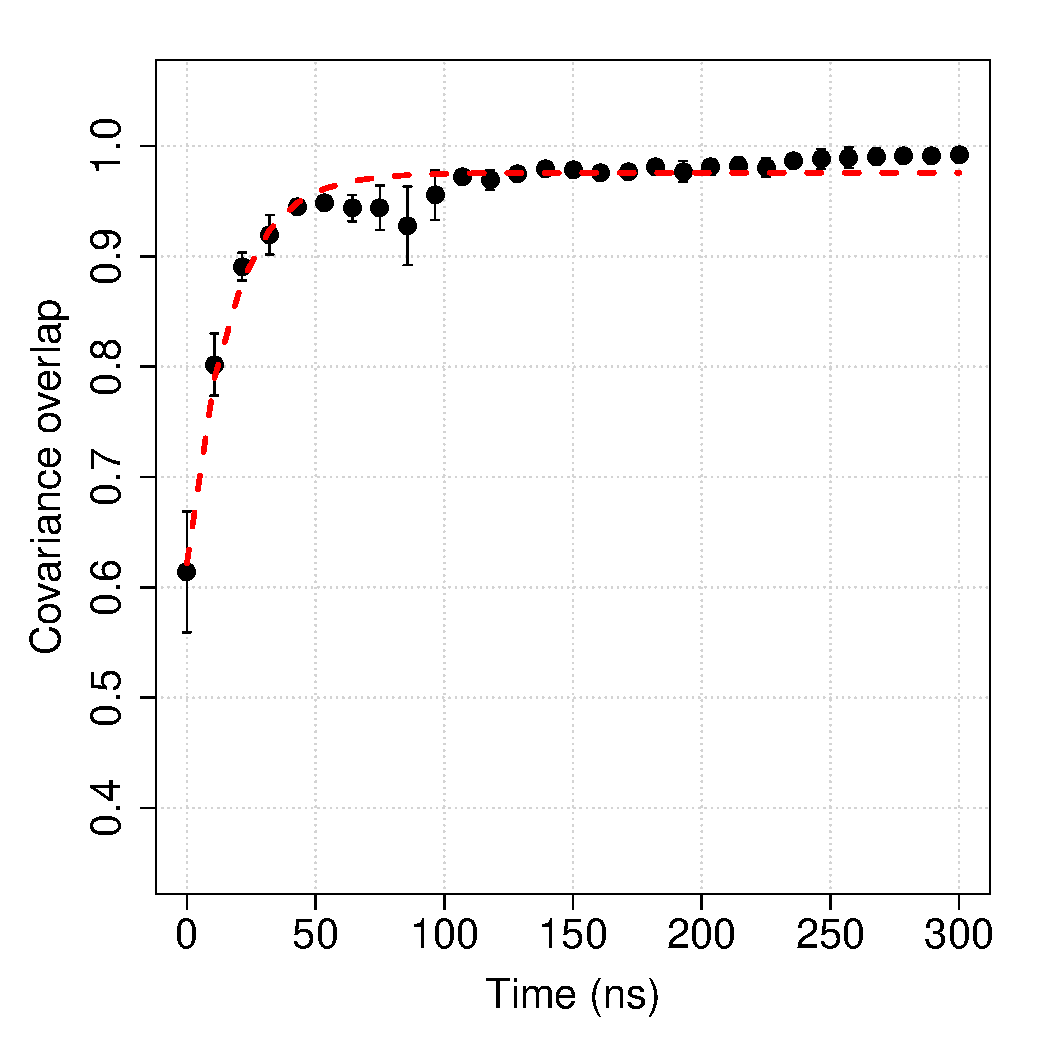
\includegraphics[width=.99\textwidth]{pos_overlap_apo.pdf}
    \caption{$C_\alpha$ positional covariance}\label{fig:4a}
  \end{subfigure}%   
  \begin{subfigure}[b]{.4\linewidth}
    \centering
    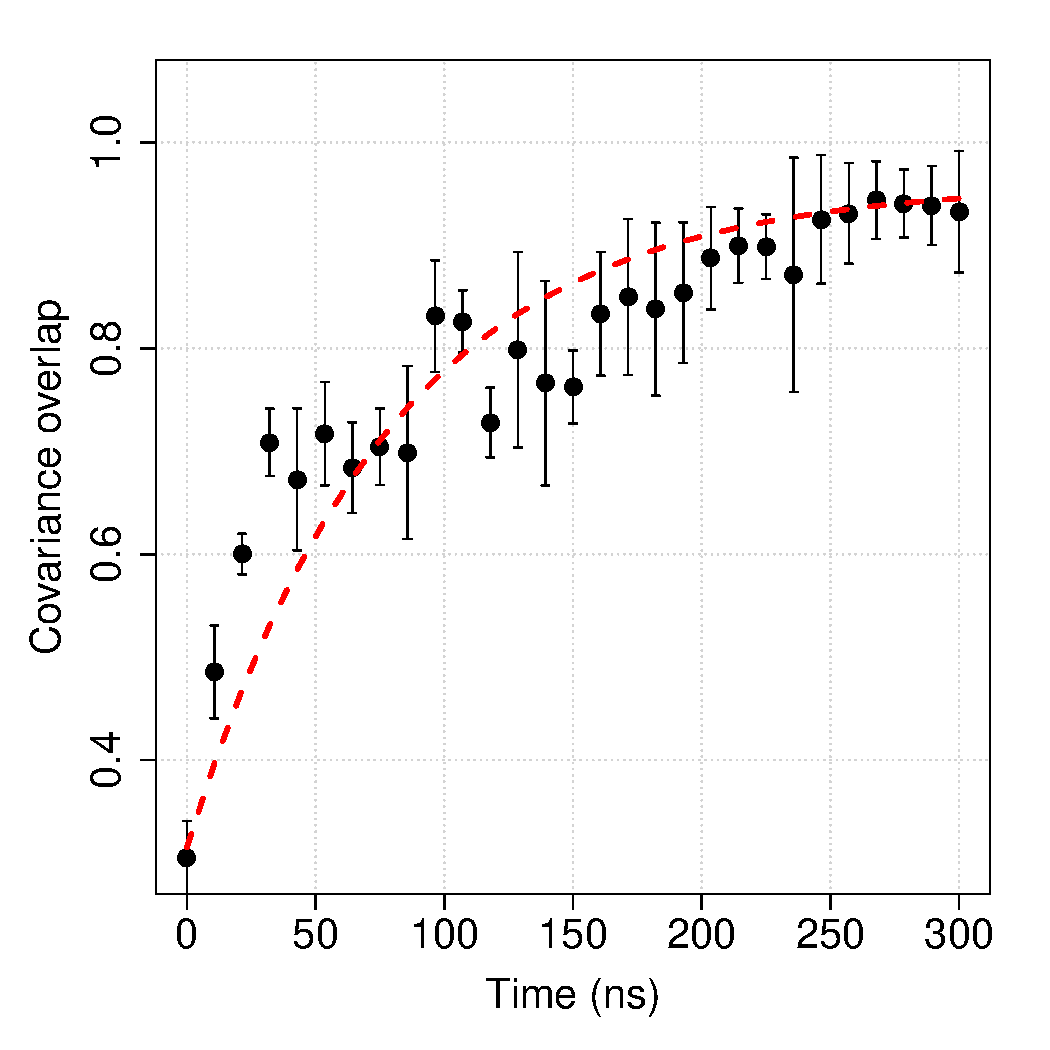
\includegraphics[width=.99\textwidth]{MI_overlap_apo.pdf}
    \caption{Mutual information}\label{fig:3b}
  \end{subfigure}%  
  \begin{subfigure}[b]{.4\linewidth}
    \centering
    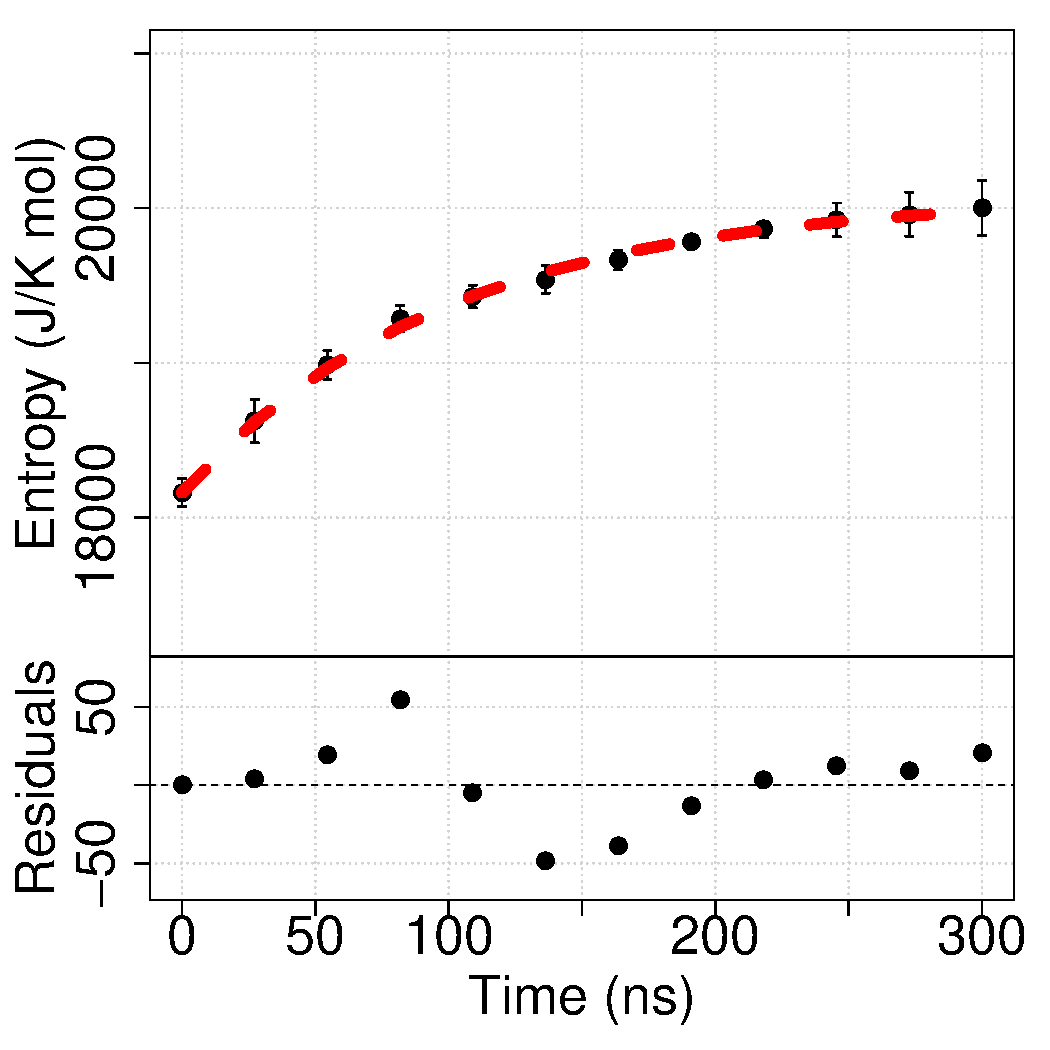
\includegraphics[width=.99\textwidth]{entropy_apo.pdf}
    \caption{Entropy}\label{fig:3b}
  \end{subfigure}%  
\caption{Energetic and structural features of apo monomeric PKM2 equilibration. Comparison of the time-averaged covariance overlap for the (a) $C_\alpha$ covariance matrix and the (b) structural alphabet mutual information matrix. The first ten eigenmodes were used in calculating covariance overlap for both (a) and (b). (c) Time-averaged configurational entropy measured over the course of the MD simulation.}\label{fig:2}
\end{figure}
\end{figure}
\begin{figure}[!ht]
\centering
\begin{subfigure}[b]{.4\linewidth}
    \centering
    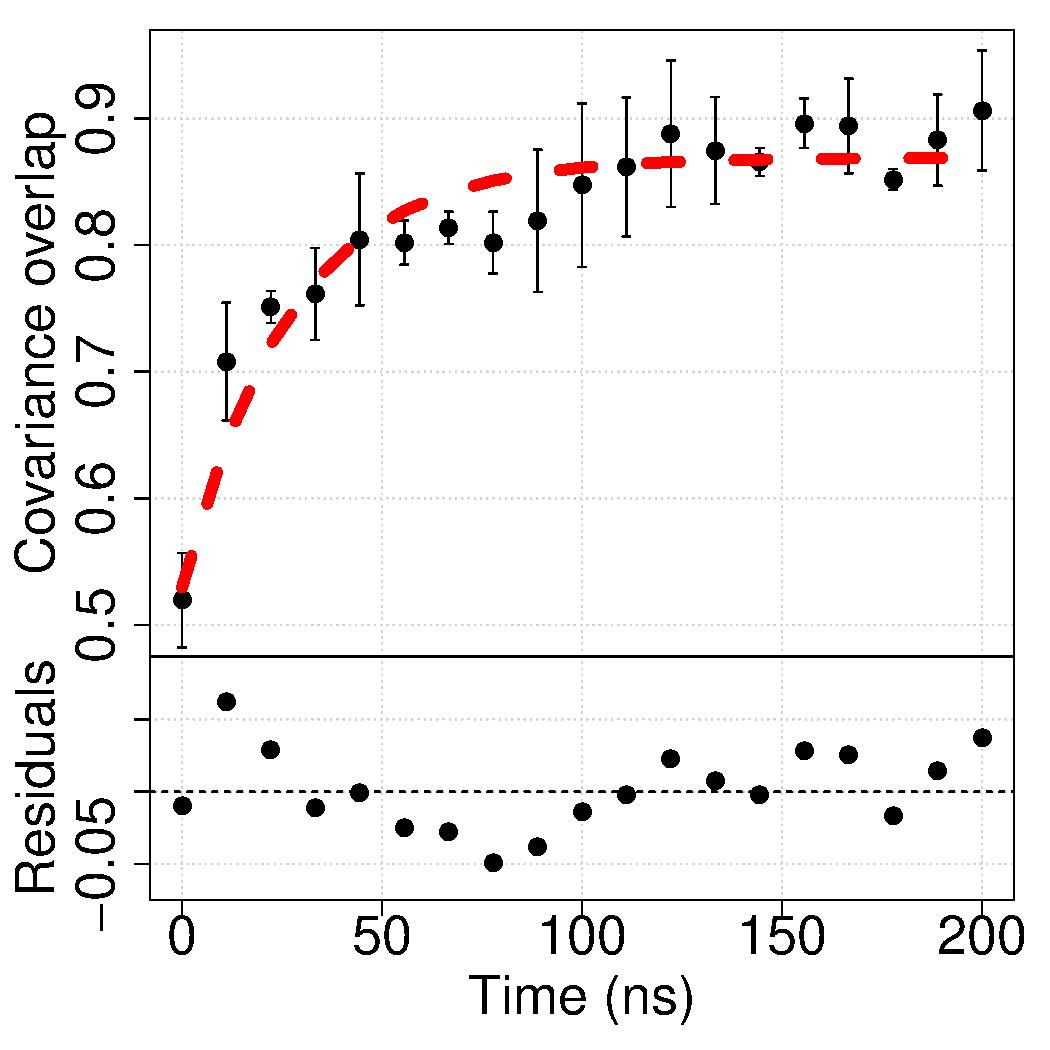
\includegraphics[width=.99\textwidth]{pos_overlap_phe.pdf}
    \caption{$C_\alpha$ positional covariance}\label{fig:4a}
  \end{subfigure}%   
  \begin{subfigure}[b]{.4\linewidth}
    \centering
    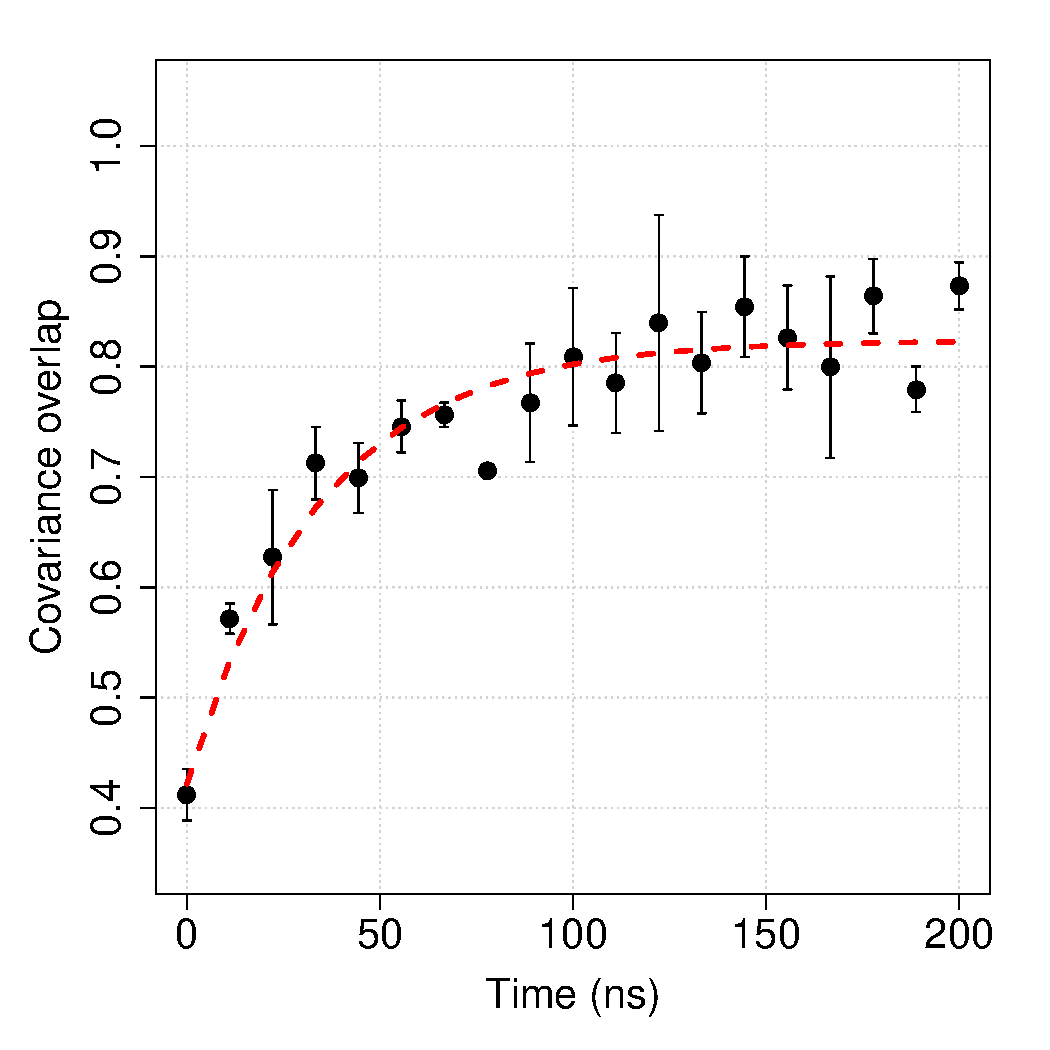
\includegraphics[width=.99\textwidth]{MI_overlap_phe.pdf}
    \caption{Mutual information}\label{fig:3b}
  \end{subfigure}%  
  \begin{subfigure}[b]{.4\linewidth}
    \centering
    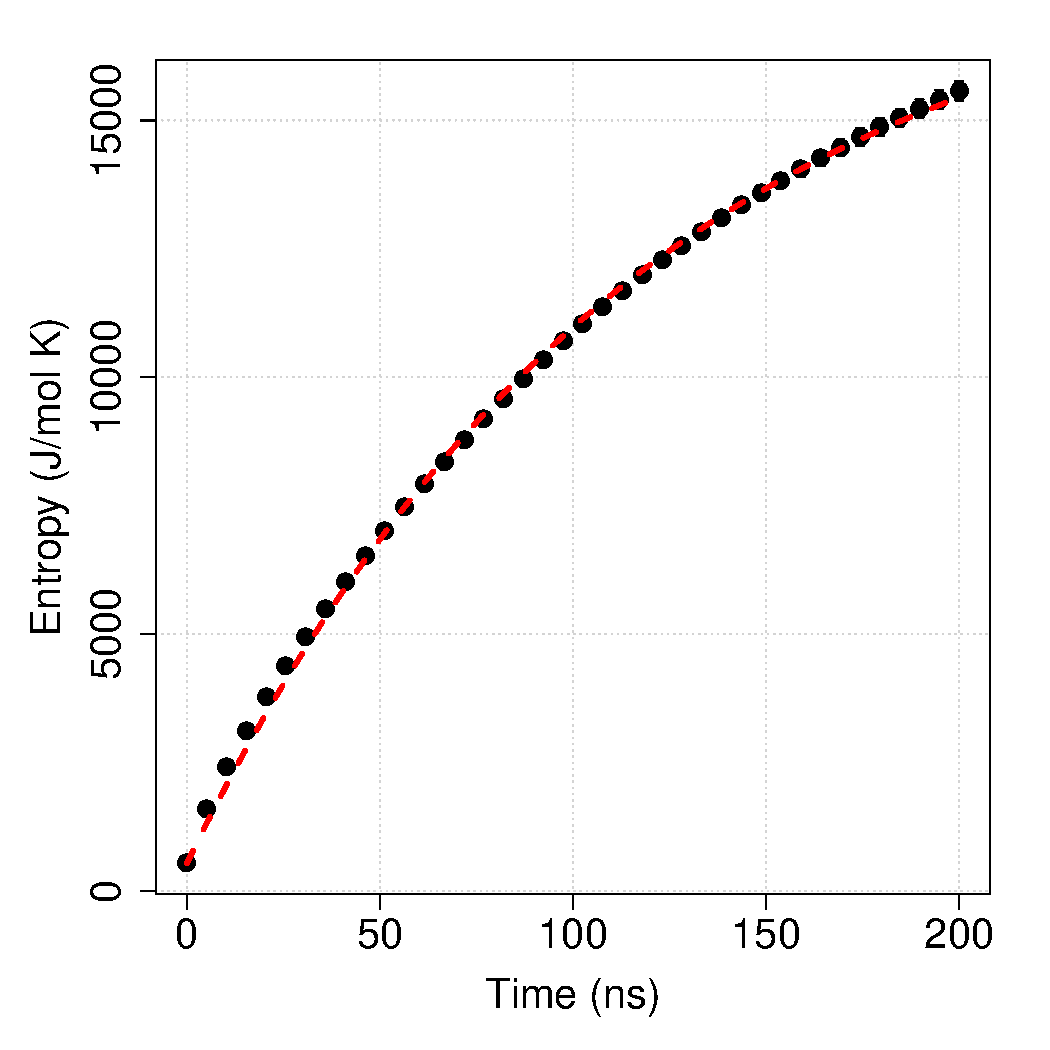
\includegraphics[width=.99\textwidth]{entropy_phe.pdf}
    \caption{Entropy}\label{fig:3b}
  \end{subfigure}%  
\caption{Energetic and structural features of monomeric PKM2 + L-phenylalanine equilibration. Comparison of the time-averaged covariance overlap for the (a) $C_\alpha$ covariance matrix and the (b) structural alphabet mutual information matrix. The first ten eigenmodes were used in calculating covariance overlap for both (a) and (b). (c) Time-averaged configurational entropy measured over the course of the MD simulation.}\label{fig:2}
\end{figure}
\begin{table}[]
\centering
\caption{Equilibration kinetics of MD simulations fit using exponential curves}
\label{my-label}
\begin{tabular}{@{}llll@{}}
\toprule
System          & Measure            & $k_1$ ($ns^{-1}$) & $t_1$ ($ns$) \\ \midrule
Apo mPKM2       & Covariance         & 0.060         & 11.56     \\
(300 $ns$)      & Mutual information & 0.012         & 57.15     \\
                & Entropy            & 0.010         & 101.30     \\ \midrule
mPKM2 + FBP     & Covariance         & 0.065         & 10.29     \\
(500 $ns$)      & Mutual information & 0.011         & 62.13     \\
                & Entropy            & 0.006         & 111.30    \\ \midrule
mPKM2 + Tepp-46 & Covariance         & 0.012         & 57.53     \\
(1000 $ns$)     & Mutual information & 0.006         & 123.70    \\
                & Entropy            & 0.003         & 272.40    \\ \midrule
mPKM2 + L-Phe   & Covariance         & 0.038         & 18.41     \\ 
(200 $ns$)      & Mutual information & 0.029         & 23.67     \\
                & Entropy            & 0.008         & 81.84     \\ \bottomrule
\end{tabular}
\end{table}
\\
\\
From the rate constants derived from time-averaged measurements of the covariance overlap of the $C_\alpha$ covariance matrix and the structural alphabet mutual information matrix, along with the time-averaged configurational entropy, it appears that the separation of distinct timescales of protein dynamics is present in each of the simulated liganded states of PKM2. From these rate constants we can assign a numerical confidence to sampling. Additionally, we  

\end{document}
 
